\documentclass[a4paper, 12pt]{article}

%%% Работа с русским языком
\usepackage{cmap}					% поиск в PDF
\usepackage{mathtext} 				% русские буквы в формулах
\usepackage[T2A]{fontenc}			% кодировка
\usepackage[utf8]{inputenc}			% кодировка исходного текста
\usepackage[russian]{babel}	% локализация и переносы

%%% Дополнительная работа с математикой
\usepackage{amsmath,amsfonts,amssymb,amsthm,mathtools} % AMS
\usepackage{icomma} % "Умная" запятая: $0,2$ --- число, $0, 2$ --- перечисление

%% Номера формул
%\mathtoolsset{showonlyrefs=true} % Показывать номера только у тех формул, на которые есть \eqref{} в тексте.

%% Шрифты
\usepackage{euscript}	 % Шрифт Евклид
\usepackage{mathrsfs} % Красивый матшрифт

%% Поля
\usepackage[left=2cm,right=2cm,top=2cm,bottom=2cm,bindingoffset=0cm]{geometry}

%% Русские списки
\usepackage{enumitem}
\makeatletter
\AddEnumerateCounter{\asbuk}{\russian@alph}{щ}
\makeatother

%%% Работа с картинками
\usepackage{graphicx}  % Для вставки рисунков
\graphicspath{{images/}{images2/}}  % папки с картинками
\setlength\fboxsep{3pt} % Отступ рамки \fbox{} от рисунка
\setlength\fboxrule{1pt} % Толщина линий рамки \fbox{}
\usepackage{wrapfig} % Обтекание рисунков и таблиц текстом

%%% Работа с таблицами
\usepackage{array,tabularx,tabulary,booktabs} % Дополнительная работа с таблицами
\usepackage{longtable}  % Длинные таблицы
\usepackage{multirow} % Слияние строк в таблице

%% Красная строка
\setlength{\parindent}{2em}

%% Интервалы
\linespread{1}
\usepackage{multirow}

%% TikZ
\usepackage{tikz}
\usetikzlibrary{graphs,graphs.standard}

%% Верхний колонтитул
\usepackage{fancyhdr}
\pagestyle{fancy}

%% Перенос знаков в формулах (по Львовскому)
\newcommand*{\hm}[1]{#1\nobreak\discretionary{}
	{\hbox{$\mathsurround=0pt #1$}}{}}

%% Мои дополнения
\usepackage{float} %Добавляет возможность работы с командой [H] которая улучшает расположение на странице
\usepackage{gensymb} %Красивые градусы
\usepackage{graphicx}               % Импорт изображений
\usepackage{caption} % Пакет для подписей к рисункам, в частности, для работы caption*

% подключаем hyperref (для ссылок внутри  pdf)
\usepackage[unicode, pdftex]{hyperref}

%%% Теоремы
\theoremstyle{plain}                    % Это стиль по умолчанию, его можно не переопределять.
\renewcommand\qedsymbol{$\blacksquare$} % переопределение символа завершения доказательства

\newtheorem{theorem}{Теорема}[section] % Теорема (счетчик по секиям)
\newtheorem{proposition}{Утверждение}[section] % Утверждение (счетчик по секиям)
\newtheorem{definition}{Определение}[section] % Определение (счетчик по секиям)
\newtheorem{corollary}{Следствие}[theorem] % Следстиве (счетчик по теоремам)
\newtheorem{problem}{Задача}[section] % Задача (счетчик по секиям)
\newtheorem*{remark}{Примечание} % Примечание (можно переопределить, как Замечание)
\newtheorem{lemma}{Лемма}[section] % Лемма (счетчик по секиям)

\begin{document}
	\newcommand{\HRule}{\rule{\linewidth}{0.7mm}} % Defines a new command for the horizontal lines, change thickness here
	
	\begin{center}
		\large\textbf{Московский Физико-Технический Институт}\\ % Name of your university/college
		\large\textbf{(государственный университет)}
	
		\vfill
		
		\Large Лабораторная работа по курсу общей физики № *labnum*\\[0.5cm] % Preambule of your document title
		
		
		\HRule
		\\[0.4cm]
		{ \huge \bfseries *name of your labwork*}% Title of your document
		\\[0.4cm] 
		\HRule
		\\[0.5cm]
		
		\ \\
	\textbf{\large Автор:} \\	
	\large *your name* *groupname*\\ % Your name and something more, your group num for example
		\vfill
		\hspace*{-0.8 cm}
\includegraphics[width=100 pt]{frkt_logo}\\ % logo of your  company/university/college
		\large Долгопрудный, 2021 % location and year
	\end{center}

\newpage
\setcounter{page}{2}
\fancyfoot[c]{\thepage}
\fancyhead[L] {Работа № *labnum*} % some information in page header
\fancyhead[R]{}
	
	
	\section*{Аннотация}
	
	\subsection*{Цель и оборудование}
	
	\begin{enumerate}
		\item \textbf{Цель работы:} изучение дифракция света на синусоидальной акустической решётке и наблюдение фазовой решётки методом тёмного поля.
		
		\item \textbf{В работе используются:} оптическая скамья, осветитель, два длиннофокусных объектива, кювета с жидкостью, кварцевый излучатель с микрометрическим винтом, генератор ультрозвуковой частоты, линза, вертикальная нить на рейтере, микроскоп.		
	\end{enumerate}    
	
	\subsection*{Теоретическое введние}	
	
	В работе используются оптическая скамья, осветитель, два длиннофокусных объектива, кювета с жидкостью, кварцевый излучатель с микрометрическим винтом, генератор звуковой частоты, линза, горизонтальная нить на рейтере, микроскоп. 
	
	При прохождении ультразвуковой волны через жидкость в ней возникают периодические неоднородности коэффициента преломления, создается фазовая решетка, которую мы считаем неподвижной ввиду малости скорости звука относительно скорости света. Показатель
	преломления n изменяется по закону:
	
	\begin{equation}\label{}
	n = n_0 (1 + m \cos \Omega x)
	\end{equation}
	
	Здесь $ \Omega = 2 \pi / \Lambda $ --- волновое число для ультразвуковой волны, $ m $ --- глубина модуляции $ n $ $ (m \ll 1 $).
	
	Положим фазу $ \phi $ колебаний световой волны на передней стенке кюветы равной нулю, тогда на задней поверхности она равна:
	
	\begin{equation}\label{}
	\phi  = k n L = \phi_0 (1 + m \cos \Omega x)
	\end{equation}
	
	Здесь $ L $ --- толщина жидкости в кювете, $ k = 2 \pi / \lambda $ --- волновое число для света.
	
	После прохождения через кювету световое поле есть совокупность плоских волн, распространяющихся под углами $ \theta $, соответствующими максимумам в дифракции Фраунгофера:
	
	\begin{equation}\label{}	
	\Lambda \sin \theta_m = m \lambda
	\end{equation}
	
	Этот эффект проиллюстрирован на рисунке 1.
	\begin{figure}[H]
		\centering	
		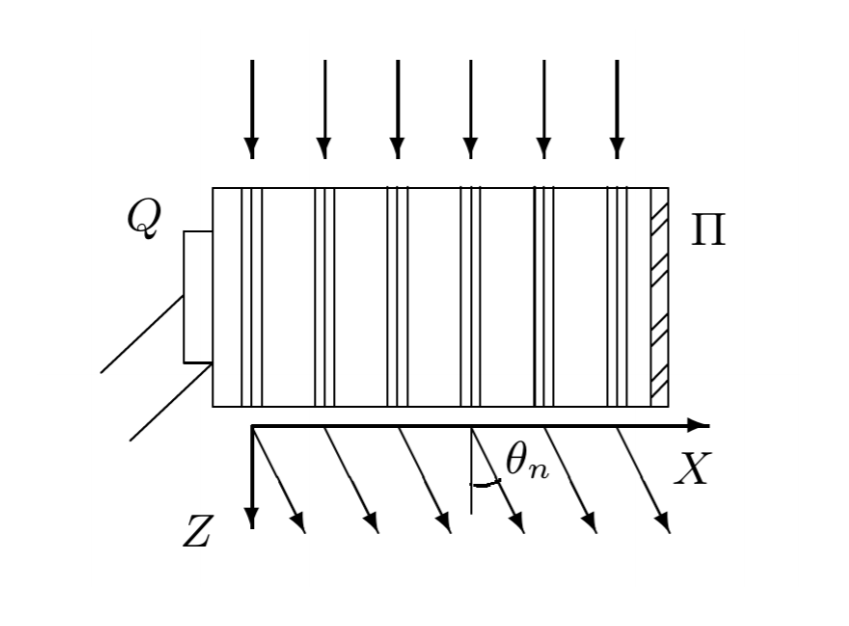
\includegraphics[scale = 0.3]{images/pic_1.png}
		\caption{Дифракция световых волн на акустической решетке}
		\label{diff}
	\end{figure}
	
	Зная положение дифракционных максимумов, по формуле (1) легко определить длину ультразвуковой волны, учитывая малость $ \theta $: $ \sin \theta \approx \theta \approx l_m /F  $, где $ l_m $ --- расстояние от нулевого до последнего видимого максимума, $ F $ --- фокусное расстояние линзы. Тогда получим:
	
	\begin{equation}\label{}
	\Lambda = m \lambda F/ l_m 
	\end{equation}
	Скорость ультразвуковых волн в жидкости, где $ \nu $ --- частота колебаний излучателя:
	
	\begin{equation}\label{}
	v = \Lambda \nu 
	\end{equation}
	
	\subsection*{Эксперементальная установка}
	
	\textbf{Схема установки. }Схема установки приведена на рисунке 2. Источник света Л через светофильтр Ф и конденсор К освещает вертикальную щель $ S $, находящуюся в фокусе объектива $ O_1 $. После объектива параллельный световой пучок проходит через кювету С перпендикулярно акустической решетке, и дифракционная картина собирается в фокальной плоскости объектива $ O_2 $ , наблюдается при помощи микроскопа М.
	
	Предварительную настройку установки произведем в соответствии с инструкцией с зеленым фильтром, далее в работе используется красный.
	
	\begin{figure}[H]
		\centering	
		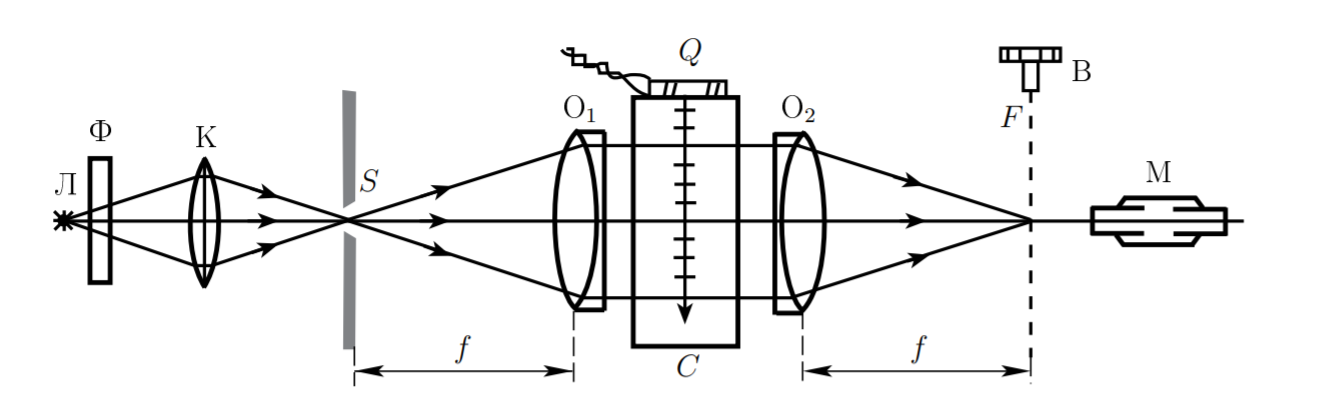
\includegraphics[scale=0.3]{images/pic_2.png}
		\caption{Схема для наблюдения дифракции на акустической решетке}
		\label{shema1}
	\end{figure}
	
	Параметры установки: фокусное расстояние объектива $F = 30 $ см, одно деление винта микроскопа составляет 20~мкм, полоса пропускания фильтра \mbox{$\lambda = 6400\pm 200$ Å}.
	
	Для определения скорости ультразвука методом темного поля будем использовать следующую установку.
	\begin{figure}[H]
		\centering	
		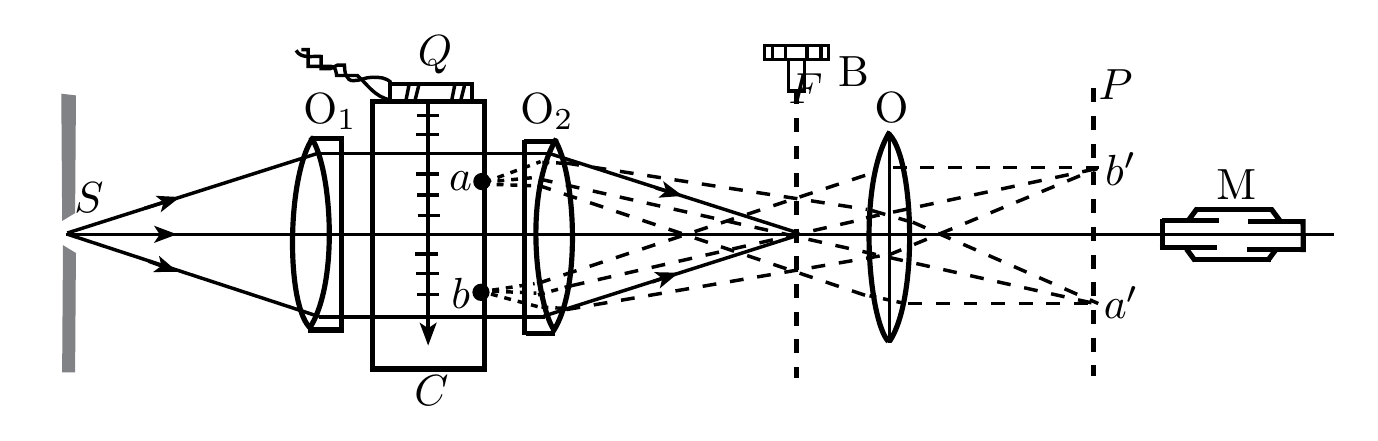
\includegraphics[scale=0.6]{pic_7.png}
		\caption{Схема для определения скорости ультразвука методом темного поля}
		\label{shema1}
	\end{figure}

	\section*{Ход работы}
\end{document}